% Section content template for individual Educative lessons
% This file contains the actual content for a specific section
% Generated from Educative API section content

% Section: Payment Service and Fraud Detection in Uber Design
% Section ID: 6353616188735488
% Section Slug: payment-service-and-fraud-detection-in-uber-design
% Generated: 2025-12-07T23:31:57.236184

Our goal in this lesson is to highlight the need to secure the system against malicious activities. We 'll discuss fraudulent activities in the context of payment. We
'll first briefly go through how the payment system works, and then we'll cover how to guard our system against malicious activity.\\
\strut \\
The payment service deals with the payments side of the Uber application. It includes collecting payment from the rider to give it to the driver. As the trip completes, it collects the trip information, calculates the cost of the journey, and initiates the payment process.\\
\strut \\

\subsection{Major functionality}\label{7y4n6gV93bnGxlHfoJd6F}
\\
The Uber payments platform includes the following functionality:

\begin{itemize}
\item
\protect\phantomsection\label{JUZ_JQPDyCovlvyQlNABj}
\textbf{New payment options}: It adds new payment options for users.
\item
\protect\phantomsection\label{9VDD3jR9fBPm-CcElrisr}
\textbf{Authorization}: It authorizes(In a payment service, authorization is a process to verify the payment method---for example, whether a certain credit card is valid or not.) the payments for transactions.
\item
\protect\phantomsection\label{15DnkFXMXXN-cBTnW_Yey}
\textbf{Refund}: It refunds a payment that was authorized before.
\item
\protect\phantomsection\label{XO5U_XqDlBkhy-9BqWEuT}
\textbf{Charging:} It moves money from a user account to Uber.
\end{itemize}

\subsection{What to prevent}\label{s4_38XyvGg3NrpWB6B1jJ}
\\
We need to prevent the following scenarios for the success of the payment system:

\begin{itemize}
\item
\protect\phantomsection\label{v1nLiI2K81mIrY0Yuqj_5}
Lack of payment
\item
\protect\phantomsection\label{TUZXUvyoN-_UTKzQqBe3j}
Duplicate payments
\item
\protect\phantomsection\label{lCc2h2D7b6f62bjEhgBOG}
Incorrect payment
\item
\protect\phantomsection\label{PGBj9Ts91C1nfTLNvD9LU}
Incorrect currency conversion
\item
\protect\phantomsection\label{RrJI7b7Tuji3UAHegxLtI}
Dangling authorization
\end{itemize}
\\
The Uber payment platform is based on the double-entry bookkeeping(Double-entry bookkeeping, also known as, double-entry accounting, is a method of bookkeeping that relies on a two-sided accounting entry to maintain financial information. Every entry to an account requires a corresponding and opposite entry to a different account. Source: Wikipedia) method.

\subsection{Design}\label{57_aeud3UcI4cLuxWCin6}
\\
Let's look at the design of the payment platform in Uber and learn how different components work together to complete the transactions:

\begin{figure}[htbp]
 \centering
 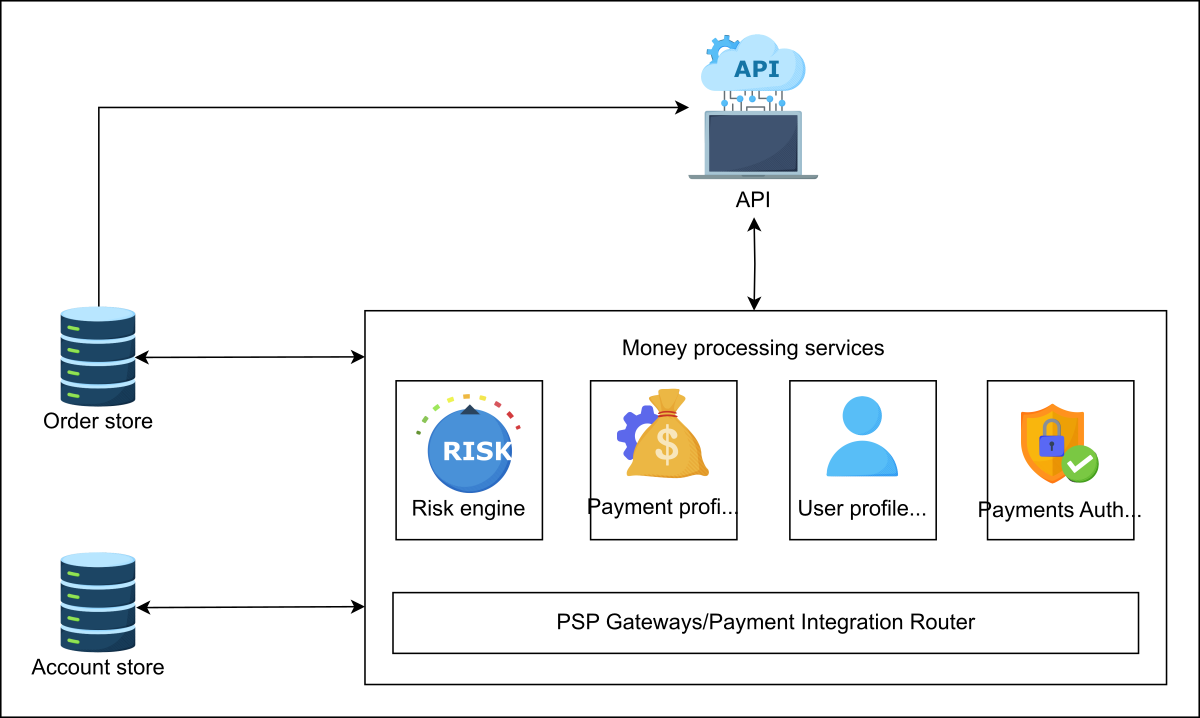
\includegraphics[width=0.5\textwidth]{Images/chapter_30/section_6353616188735488/5099564886786048.png}
 \caption{The payment platform in Uber}
\end{figure}

The key components used in the payment service are as follows:

\begin{itemize}
\item
\protect\phantomsection\label{uJh7N0A3wncsK9LVfjddu}
\textbf{API}: The Uber API is used to access the payment service.
\item
\protect\phantomsection\label{shtIXlmZPi14HG937vtNe}
\textbf{Order store}: This stores all the orders. Orders collect payments and contain information regarding money flow between different riders and drivers.
\item
\protect\phantomsection\label{FiIxBZH5RU0MQj_LPG9HC}
\textbf{Account store}: This stores all the accounts of riders and drivers.
\item
\protect\phantomsection\label{tZ4lUxvJNm8x__3cI39PP}
\textbf{Risk engine}: The risk engine analyzes different risks involved in collecting payment from a particular rider. It checks the history of the rider---for example, the rating of the rider, if the rider has sufficient funds in their rider account, any pending dues, if the rider cancels the rides frequently, and so on.
\item
\protect\phantomsection\label{TJU1srTVb7Wdlr61Yl7Es}
\textbf{Payment profile service}: This provides information on the payment mechanisms, such as credit and debit cards.
\item
\protect\phantomsection\label{OSGq4Ne4d4yWlXpGMWsgE}
\textbf{User profile service}: This provides information regarding users' payments.
\item
\protect\phantomsection\label{TIGeWXoGy-qoV2CP0T1si}
\textbf{Payment authorization service}: This offers payment authentication services.
\item
\protect\phantomsection\label{mxNmZIVmIcRb05C5P2Fb1}
\textbf{PSP gateways}: This connects with payment service providers
\end{itemize}

\subsubsection{Workflow}\label{5Yrvo3BXtKOqHCM46oMgn}
\\
The following steps show the workflow of the payment service:

\begin{enumerate}
\item
\protect\phantomsection\label{__0vEhj7kyKc7SVByClOz}
When a rider requests a ride, the Uber application uses the Uber API to request the risk engine to check the risks involved.
\item
\protect\phantomsection\label{Ig_Mi90ZFOO5J_AseCwEP}
The risk engine obtains user information from the user profile service and evaluates the risk involved.
\item
\protect\phantomsection\label{CNm_4vzkkYkl2ViJA2qhe}
If the risks are high, the rider's request isn't entertained.
\item
\protect\phantomsection\label{KyG4HP3ztvC4pn8AMjmez}
If the risks are low, the risk engine creates an authorization token and sends it to the payment profile service (for record-keeping), which fetches that token and sends it to the payment authorization service.
\item
\protect\phantomsection\label{UhZv-2VJrrx5uI4OARESo}
The payment authorization service sends that request to the PSP gateway, which contacts the service provider for authorization.
\item
\protect\phantomsection\label{GzAGaSjzeASxGfrFR3PDe}
The PSP gateway sends the authorization token back to the payment authorization service, which sends the token back to the Uber application that the trip request is approved.
\item
\protect\phantomsection\label{aiwVrmMkV0IjOr8w-bdwR}
After the trip is completed, the Uber application uses the API to send the payment request to the PSP gateway with authorization data.
\item
\protect\phantomsection\label{MiGgmqyUtpg2qXAqtfqrm}
The PSP gateway contacts the service provider and sends the status back to the Uber application through the API.
\end{enumerate}
\\
The Uber payment service is constructed with a set of microservices grouped together as a stream-processing architecture.

\subsubsection{Apache Kafka}\label{PAG7v7LC-1WjaGss2nSrT}
\\
\textbf{Kafka} is an open-source stream-processing(Stream processing is a computer programming paradigm that simplifies parallel software and hardware by restricting the parallel computation that can be performed. Given a sequence of data (a stream), a series of operations (kernel functions) is applied to each element in the stream. Source: Wikipedia) software platform. It's the primary technology used in payment services. Let's see how Kafka helps to process an order:

\begin{figure}[htbp]
 \centering
 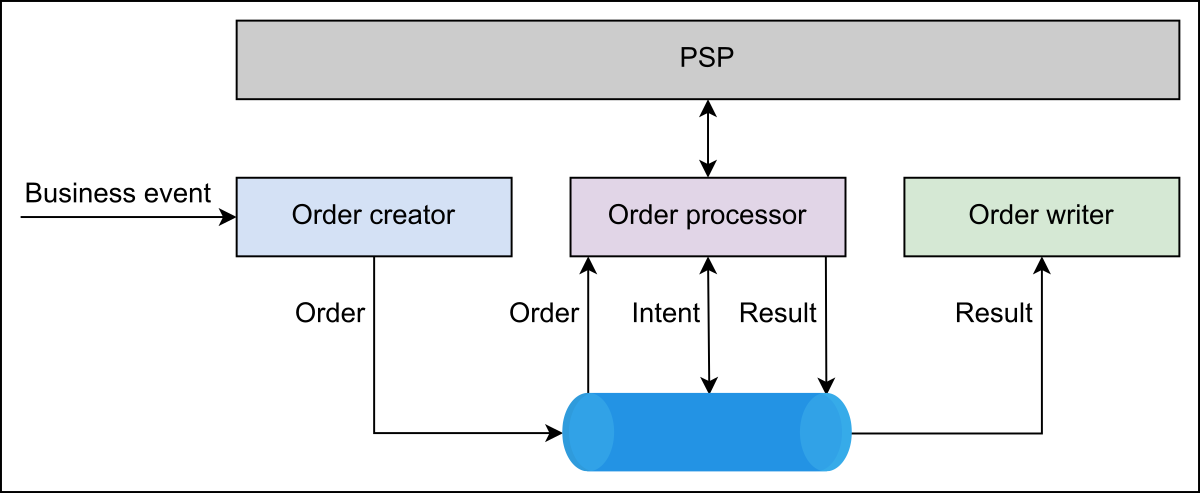
\includegraphics[width=0.5\textwidth]{Images/chapter_30/section_6353616188735488/5455818918723584.png}
 \caption{Payment service with Kafka}
\end{figure}

The order creator gets a business event---for example, the trip is finished. The order creator creates the money movement information and the metadata. This order creator publishes that information to Kafka. Kafka processes that order and sends it to the order processor. The order processor then takes that information from Kafka, processes it, and sends it as intent to Kafka. From that, the order processor again processes and contacts the PSP. The order processor then takes the answer from PSP and transmits it to Kafka as a result. The result is then saved by the order writer.
\\
The key capabilities of Kafka that the payment service uses are the following:

\begin{itemize}
\item
\protect\phantomsection\label{uywjx6v6yP6EXPCFYHxa-}
It works like message queues to publish and subscribe to message queues.
\item
\protect\phantomsection\label{y6SVZSz6K3EGIjXFJvZOn}
It stores the records in a way that is fault tolerant.
\item
\protect\phantomsection\label{Nl8f1bBf06JtoaVTxR1Fc}
It processes the payment records asynchronously.
\end{itemize}

\subsection{Fraud detection}\label{s1xif_tEYmqsAWl_eVfxY}
\\
Fraud detection is a critical operational component of our design. Payment fraud losses are calculated as a percentage of gross amounts. Despite fraud activities accounting for a tiny portion of gross bookings, these losses considerably influence earnings. Moreover , if malicious behavior isn't promptly detected and handled, it may be further leveraged, which results in significant losses for the business. Earlier
, we discussed the risk engine that detects fraud before the trip starts. Here , we'll focus on the fraud detection that happens during trips or at the end of the trips.
\\
Fraud detection is challenging because many instances of fraud are like detecting zero-day security bugs. Therefore, our system needs intelligence to detect anomalies, and it also needs accountability for automated decisions in the form of human-led audits.
\\
The activities(The following list of eight fraudulent activities is taken from: https://www.uber.com/gb/en/drive/driver-app/fraud-activities/) that are considered fraudulent by Uber are as follows:

\begin{itemize}
\item
\protect\phantomsection\label{hGAECLLBt2R-nnsdgn5gh}
A driver deliberately increases the time or distance of a trip in a dishonest manner---for example, if they take a much longer route than necessary to the rider's destination.
\item
\protect\phantomsection\label{k8vj4Dz3dmUBGdP_8HNjT}
A driver manipulates the GPS data or uses fake location GPS apps.
\item
\protect\phantomsection\label{26SIGrSB2_SiSVEXFTJia}
A driver confirms trips with no intention of completing them, forcing riders to cancel.
\item
\protect\phantomsection\label{UNTuPlXZpSf66xa33dOCN}
A driver creates false driver or rider accounts for fraudulent purposes.
\item
\protect\phantomsection\label{Rl2VBnRVsZdfWwu4nWCOH}
A driver provides incorrect or inaccurate information about themselves when opening their account.
\item
\protect\phantomsection\label{mLs6Nd3evpOLWH0uqfy-z}
A driver drives a vehicle that hasn't been approved by Uber.
\item
\protect\phantomsection\label{4jOCjJLIBm2E3cI_pd-CV}
A driver claims fraudulent fees or charges, such as unwarranted cleaning fees.
\item
\protect\phantomsection\label{SCVUGcmZ6FLgMl-2AFFlj}
A driver willfully confirms or completes fraudulent trips.
\end{itemize}

\subsubsection{RADAR}\label{dcVoSWpoks4B5PsRP2RMp}
\\
Uber introduced \textbf{RADAR}, a human-assisted AI fraud detection and mitigation solution to handle the discussed scenarios of fraud. The RADAR system detects fraud by analyzing the activity time series of the payment system. It then generates a rule for it and stops it from further processing. This proactive approach can help to detect unseen fraud in real time. This detection model also uses human knowledge for continuous improvements. Here, we'll briefly discuss how RADAR works:

\begin{figure}[htbp]
 \centering
 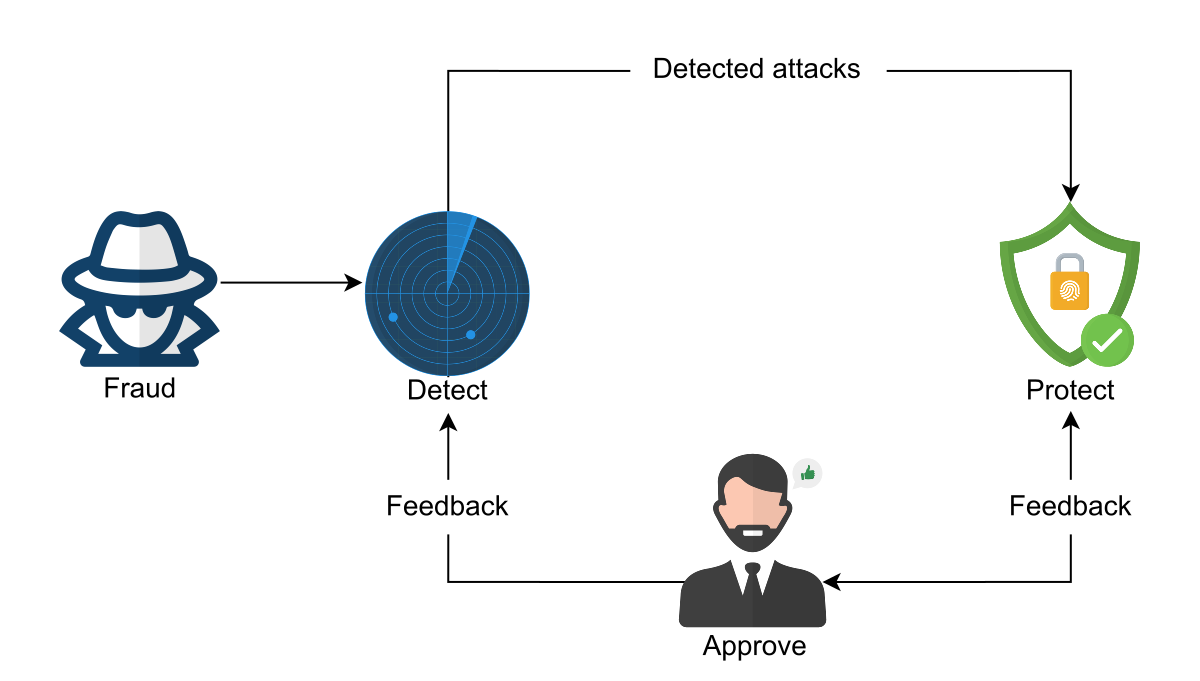
\includegraphics[width=0.5\textwidth]{Images/chapter_30/section_6353616188735488/5783323125481472.png}
 \caption{The RADAR fraud detection solution}
\end{figure}

RADAR recognizes the beginning of a fraud attempt and creates a rule to prevent it. The fraud analyst is involved in the next step. They review the rule and approve or reject it if required. They then send feedback (approved or not approved) to the protection system. The feedback is also sent to the fraud detection system by the fraud analysts to improve detection.
\\
Furthermore, the system examines the data in the following time dimensions:

\begin{itemize}
\item
\protect\phantomsection\label{dfiuR4-Zny90GPdw8LMLI}
It examines the trip time when a trip has been completed. Multiple factors are involved in real-time trip monitoring. For instance, the system can check whether or not the driver and rider locations are the same. The system can also monitor the speed and analyze the real traffic to check if the driver is intentionally driving slow or if there's traffic congestion.
\item
\protect\phantomsection\label{DTjhI57WhqtnfGw8AOASF}
Payment settlement time refers to obtaining payment processing data. It might take days or weeks to settle.
\end{itemize}
\\
We've just discussed the basic details of how guarding against malicious activity at scale is necessary for the success of a business. In the proposed model, the human experts are involved, potentially decreasing the scalability of the system. Research is being carried out on how to ensure that the decisions made by the AI system are fair and ethical.

% End of section content